
%----------------------------------------------------------------------------------------
%	Lecture 12
%----------------------------------------------------------------------------------------

\chapter{Double Integrals in Polar Coordinates}

\bigbreak

We've seen how to compute double integrals by dividing the region into many little rectangles.
And taking the limit as the rectangles get smaller and smaller.

In polar coordinates, we denote at point by $(r, \theta)$ where $r$ is the distance from the origin and $\theta$ is the angle with the positive X-axis.
We have the relation $x = r \cos \theta$ and $y = r \sin \theta$.
In polar coordinates, we will slice our region by fixiing $\theta = \theta_0$.

We will take the region circle $r <= 1$ in the first quadrant.
This means that for a given $\theta = \theta_0$ the range of $r$ is $r = 0$ to $r = 1$.

\begin{figure}[ht!]
    \centering
    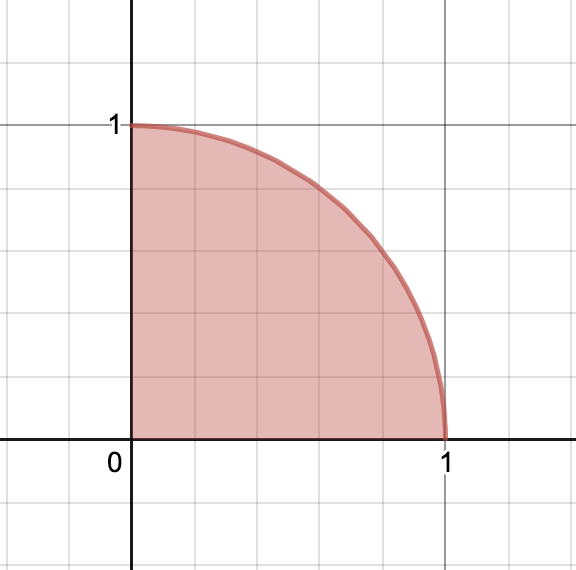
\includegraphics[scale=0.5]{./images/lecture_12_figure_1.png}
    \caption{The region $r <= 1$ in the first quadrant}
\end{figure}

Here we will integrate with $r$ first because that is usually easier.
In polar coordinates, the area element $dA$ is not $dr d\theta$ but  $dA = dr r d\theta$.
So our final integration looks like $$ \iint f(r, \theta) dA = \iint f(r, \theta) r dr d\theta$$.

Now if $f(x, y) = 1 - x^2 - y^2 = 1 - r^2$ because $x^2 + y^2$ is square of the distance of from the origin.
Thus, 
$$
\int_0^{\frac{\pi}{2}} \int_0^1 (1-r^2) r dr d\theta
 = \int_0^{\frac{\pi}{2}} \left[ \frac{r^2}{2} - \frac{r^4}{4} \right]_0^1 d\theta
 = \int_0^{\frac{\pi}{2}} \frac{1}{4} d\theta = \frac{\pi}{8}
$$

This is a lot easier than using the cartesian coordinates.
In general, there will be tradeoff between complexity of the function and the bounds of the integral.

